\section{Paso 2: datos y modelo conceptual}
\label{sec:paso2-datos-modelo-conceptual}
% Origen: 01-definicion-del-caso.md §3 y §8, 02-modelo-anylogic.md §7, 07-plan-tpi.md §5 y 09-pedidos-de-datos.md.

\subsection{Fuentes de datos}

\subsubsection{Validaciones por molinete (SBASE)}

La fuente cuantitativa principal es el dataset abierto \emph{Subte: Viajes Molinetes}
\parencite{sbase2026molinetes}. Tiene una fila por molinete y por ventana de 15 minutos, con la línea, la
estación, el identificador del molinete y los pasajeros por tipo de pago. El identificador distingue los
dos vestíbulos de Constitución:
\begin{center}
\small
\begin{tabular}{@{}ll@{}}
Vestíbulo Principal & \texttt{LineaC\_Constitucion\_Turn\textit{NN}} \\
Vestíbulo Plaza & \texttt{LineaC\_Constitucion\_Plaza\_Turn\textit{NN}} \\
\end{tabular}
\end{center}
Por eso la unidad del dato coincide con la unidad de servicio del modelo: el molinete.

El procesamiento, reproducible con el script \texttt{sbase-perfil.py} del repositorio, hizo cuatro cosas:
\begin{enumerate}
  \item \textbf{Normalizó el campo horario.} En marzo y abril de 2026 viene como \texttt{HH:MM} y en el
        resto de los meses como \texttt{HH:MM:SS}. Sin normalizar, cada hora se parte en dos grupos y los
        totales salen mal sin ningún aviso.
  \item \textbf{Excluyó los días atípicos.} Se descartaron los días cuyo flujo diario quedó por debajo del
        50~\% de la mediana. Los días excluidos coinciden uno a uno con feriados y fines de semana largos,
        lo que valida el criterio.
  \item \textbf{Fijó el período representativo.} Se usaron los días hábiles de marzo a junio de 2026:
        80 días útiles. Enero y febrero se descartaron porque son meses de vacaciones con menor carga.
  \item \textbf{Separó los vestíbulos.} El Principal tiene 22 identificadores: \texttt{Turn07} y de
        \texttt{Turn09} a \texttt{Turn29}. \texttt{Turn07} registró 3 pasajeros en seis meses, por lo que
        en la práctica hay 21 molinetes con tráfico. Por ventana se observan en promedio 19,5 molinetes
        activos.
\end{enumerate}

La tabla~\ref{tab:perfil} y la figura~\ref{fig:perfil} muestran el perfil resultante. El total medio de
la franja es de \num{18532} validaciones por día hábil, con el pico entre las 08:15 y las 08:45. La carga
entre molinetes es muy desigual. Entre enero y junio, \texttt{Turn14} procesó \num{1485} pasajeros por
día hábil en la franja y \texttt{Turn23}, 129: un factor de 11.

\begin{table}[H]
\centering
\caption{Validaciones medias del vestíbulo Principal por ventana de 15 minutos (días hábiles de marzo a junio de 2026, $n = 80$)}
\label{tab:perfil}
\small
\begin{tabular}{@{}lrrrrrrrrrr@{}}
\toprule
Ventana & 07:00 & 07:15 & 07:30 & 07:45 & 08:00 & 08:15 & 08:30 & 08:45 & 09:00 & 09:15 \\
\midrule
Pasajeros & \num{1544} & \num{1681} & \num{1804} & \num{1986} & \num{1873} & \num{2214} & \num{2148} & \num{1862} & \num{1700} & \num{1721} \\
\bottomrule
\end{tabular}

\vspace{2pt}
{\footnotesize Fuente: elaboración propia sobre \textcite{sbase2026molinetes}.}
\end{table}

\begin{figure}[H]
\centering
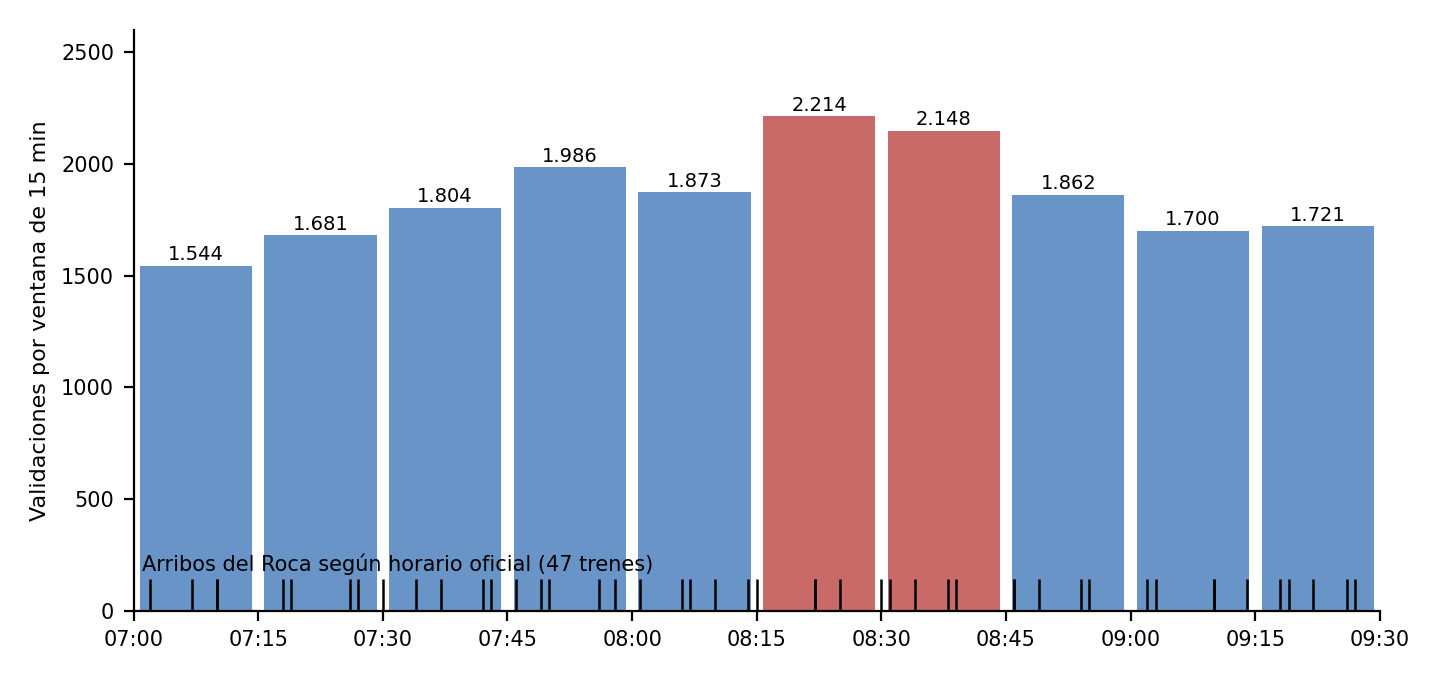
\includegraphics[width=\textwidth]{tpi-subte-perfil-demanda.png}
\caption{Validaciones medias por ventana en el vestíbulo Principal (barras; en rojo, el pico) y arribos de
los trenes del Roca a Plaza Constitución según el horario oficial (marcas). Elaboración propia sobre
\textcite{sbase2026molinetes} y \textcite{trenes2026roca}.}
\label{fig:perfil}
\end{figure}

El dato tiene dos límites, y ambos condicionan el modelo:
\begin{itemize}
  \item \textbf{Cuenta validaciones, no arribos ni esperas.} No dice cuánta gente esperó ni cuánto
        tiempo. Si en algún momento los molinetes se saturan, el conteo mide la capacidad de los
        molinetes y no la demanda real (censura por capacidad).
  \item \textbf{Es un agregado de 15 minutos.} Dentro de cada ventana se borra la estructura de las
        oleadas, que es justamente lo que genera la cola.
\end{itemize}

\subsubsection{Horario del Roca}

La estructura temporal de las oleadas se obtuvo del horario oficial de la línea Roca, vigente desde el
03/08/2026 \parencite{trenes2026roca}. Se procesaron los cuatro cuadros horarios que llegan a Plaza
Constitución: La Plata, Bosques, Glew/A.~Korn y Ezeiza/Cañuelas. De cada uno se tomaron la sección de
lunes a viernes, los trenes con destino Constitución y el horario de llegada. Se descartaron las
lanzaderas que no llegan a la terminal y se controló que un tren repetido en dos cuadros tuviera el mismo
arribo. Quedan 47 trenes entre las 07:00 y las 09:30, uno cada 3 minutos en mediana, con huecos de hasta
8 minutos. Cuatro pares de trenes llegan en el mismo minuto.

El horario fija cuándo llega cada oleada, pero no cuántas personas trae ni qué parte de ellas va a la
Línea~C.

\subsubsection{Pedidos de información pública}

Lo que ningún dataset publica se pidió a los organismos responsables. El 23/09/2026 se enviaron correos
a SBASE, a Emova (la concesionaria) y a Trenes Argentinos. El 05/10 se presentaron pedidos formales:
\begin{itemize}
  \item a SBASE, por la Ley~104 de la Ciudad: el plano de los vestíbulos, la correspondencia entre
        identificadores y equipos, el criterio de habilitación de molinetes y los tiempos de validación;
  \item a Trenes Argentinos Operaciones, por la Ley~\num{27275}: el plano de la estación, los pasajeros
        por tren, las llegadas efectivas y los estudios de trasbordo.
\end{itemize}

Trenes Argentinos respondió el 26/10/2026 \parencite{sofse2026nota}. Envió:
\begin{itemize}
  \item el plano de la estación ferroviaria en DWG, que no incluye los accesos de la Línea~C;
  \item la llegada real de cada tren entre el 02/03 y el 30/06/2026, de 07:00 a 09:30;
  \item una matriz origen-destino de la línea Roca para el mismo período.
\end{itemize}
Informó además que no existen estudios de trasbordo hacia el subte. Estos datos llegaron después de las
corridas de producción, por lo que se usan en la validación (sección~\ref{sec:paso6-validacion}) y no como
entradas. SBASE prorrogó su plazo de respuesta. \pendiente{actualizar si SBASE responde antes de la entrega.}

\subsection{Parámetros sin dato publicado}

Cuatro parámetros no surgen de ningún dato disponible: el tiempo de validación, la dispersión con que el
pasaje de un tren llega al vestíbulo, la demora entre el arribo del tren y la llegada del primer pasajero,
y la proporción de la demanda que llega en tren. Para cada uno se definió un rango con fuente, con un
valor intermedio para la comparación principal (tabla~\ref{tab:parametros}). Los contextos se ordenan por
congestión: el optimista combina servicio corto, oleadas dispersas y menos demanda en tren; el pesimista,
lo contrario.

\begin{table}[H]
\centering
\caption{Parámetros sin dato publicado: rangos y fuentes}
\label{tab:parametros}
\small
\begin{tabularx}{\textwidth}{@{}>{\raggedright\arraybackslash}p{2.6cm} >{\raggedright\arraybackslash}p{2.0cm} >{\raggedright\arraybackslash}p{2.0cm} >{\raggedright\arraybackslash}p{2.0cm} X@{}}
\toprule
Parámetro & Optimista & Intermedio & Pesimista & Fuente y carácter \\
\midrule
Tiempo de validación (s) & Triangular (1,5; 2,0; 3,0) & Triangular (1,8; 2,4; 3,5) & Triangular (2,2; 3,0; 4,5) &
Moda: 2,4~s con tarjeta inteligente en Londres; 2,6 a 2,9~s en Nueva York \parencite[Exh.~10-27]{tcqsm2013}.
Cota del propio dataset: hasta 246 pasajeros en 15 minutos por molinete, o sea una media sostenida
$\le 900/246 = 3{,}66$~s. Asimetría a la derecha por fallas de lectura [supuesto] \\
Dispersión de la descarga (s) & 220 & 145 & 110 &
Recorrido entre el primer y el último coche de una formación de 7 coches, unos 138~m [supuesto], a 0,63,
0,95 y 1,25~m/s \parencite{tcqsm2013}. Una descarga corta concentra la oleada y genera más cola \\
Demora andén--vestíbulo (s) & 84 & 106 & 159 &
$D/v + h/v_e$ con $D = 85$~m, mediana del recorrido desde los paragolpes de las 14 vías hasta la boca de
la Línea~C (rango 69 a 112~m, \cite{osm2026}), y $h = 5$~m de desnivel [supuesto] \\
Proporción que llega en tren & 0,70 & 0,80 & 0,90 &
Supuesto explícito: no hay estudio publicado de trasbordo del Roca a la Línea~C, y Trenes Argentinos
confirmó que no lo tiene \parencite{sofse2026nota} \\
\bottomrule
\end{tabularx}
\end{table}

La demora solo desplaza las oleadas en el tiempo, sin cambiar su forma, por lo que se fija en el valor
intermedio. Los otros tres parámetros moldean la congestión y son los candidatos al análisis de
sensibilidad.

La velocidad de marcha se toma uniforme entre 1,1 y 1,5~m/s, el rango que \textcite{li2024} reportan en
la literatura y dentro del cual cae su valor calibrado de 1,37~m/s. El diámetro del peatón se fijó en 0,5~m.
Es un supuesto: ninguno de los estudios citados lo informa.

\subsection{Modelo conceptual}

\textbf{Entidades.} Cada pasajero es un agente con su velocidad, su instante de ingreso, su tiempo de
validación y su molinete elegido. Los molinetes son servidores paralelos, cada uno con su propia cola.

\textbf{Generación de la demanda.} La demanda de cada ventana $k$ es la media observada $d_k$. Una
fracción $p$ (la proporción que llega en tren) se reparte en partes iguales entre los trenes cuyo pasaje
ingresa al vestíbulo en esa ventana, es decir, con arribo $+$ demora dentro de la ventana. Así, los trenes
del pico traen más gente que los del borde de la franja. El pasaje de cada tren ingresa por el acceso
desde el hall ferroviario de forma pareja durante la dispersión de la descarga. El resto, $(1-p)\,d_k$,
entra desde la calle con llegadas de Poisson no homogéneas a la tasa de cada ventana. Solo se generan
ingresos antes de las 09:30.

\textbf{Servicio y elección de molinete.} Cada pasajero elige, entre los molinetes habilitados, el que
minimiza un costo: el desvío lateral respecto de su recorrido, convertido a tiempo a 1,3~m/s, más la
espera estimada (pasajeros ya asignados a ese molinete por el tiempo de validación de referencia). La
literatura indica que la cercanía pesa fuerte \parencite{seriani2025,tian2026} y que la fila también
cuenta \parencite{wang2024}. La regla combina ambos efectos. Luego el pasajero camina hasta la cola, espera
según el orden de llegada, valida y sigue hacia las escaleras de la Línea~C.

\textbf{Horizonte.} El sistema es terminal. Cada réplica representa un día hábil de 07:00 a 09:30 y,
después del cierre de ingresos, sigue hasta que sale el último pasajero que ingresó antes de las 09:30.
Así ninguna espera queda censurada. La unidad de tiempo es el segundo, con $t = 0$ a las 07:00.

La figura~\ref{fig:conceptual} resume el flujo.

\begin{figure}[H]
\centering
\resizebox{\textwidth}{!}{%
\begin{tikzpicture}[
  caja/.style={draw, rounded corners=2pt, align=center, font=\small, minimum height=9mm, inner sep=4pt},
  dato/.style={draw, dashed, align=center, font=\footnotesize, inner sep=3pt},
  flecha/.style={-{Stealth[length=2.2mm]}}
]
\node[dato] (roca) at (0, 1.0) {Horario del Roca\\(47 trenes)};
\node[dato] (sbase) at (0, -1.0) {Perfil SBASE\\por ventana};
\node[caja] (tren) at (3.4, 1.0) {Pasaje en tren\\$p \cdot d_k$};
\node[caja] (calle) at (3.4, -1.0) {Calle, Poisson\\$(1-p)\,d_k$};
\node[caja] (hall) at (7.4, 0) {Caminata por\\el vestíbulo};
\node[caja] (eleccion) at (10.0, 0) {Elección de\\molinete};
\node[caja] (cola) at (12.5, 0) {Cola y\\validación};
\node[caja] (salida) at (12.5, -1.8) {Escaleras a\\la Línea~C};
\draw[flecha] (roca) -- (tren);
\draw[flecha] (sbase) -- (tren.south west);
\draw[flecha] (sbase) -- (calle);
\draw[flecha] (tren.east) -- (hall.north west);
\draw[flecha] (calle.east) -- (hall.south west);
\draw[flecha] (hall) -- (eleccion);
\draw[flecha] (eleccion) -- (cola);
\draw[flecha] (cola) -- (salida);
\end{tikzpicture}%
}
\caption{Modelo conceptual. Las oleadas salen del horario del Roca y el volumen, del perfil de SBASE. El
pasaje de cada tren llega con una demora y se dispersa durante la descarga. Cada pasajero elige molinete
según la distancia y la cola.}
\label{fig:conceptual}
\end{figure}

\subsection{Supuestos}

Además de los rangos de la tabla~\ref{tab:parametros}, el modelo adopta estos supuestos:
\begin{enumerate}
  \item La cola está vacía a las 07:00.
  \item Los molinetes funcionan solo en sentido de ingreso durante la franja, y los habilitados están
        disponibles todo el período.
  \item Nadie abandona la cola ni cambia de molinete una vez elegido.
  \item El volumen de cada ventana es la media de los días hábiles; todas las réplicas usan el mismo perfil.
  \item Los trenes llegan a la hora del horario oficial.
  \item El vestíbulo tiene la geometría hipotética descripta en la sección~\ref{sec:paso4-construccion-verificacion},
        porque el plano oficial no está disponible.
\end{enumerate}
Los supuestos 4 y 5 se discuten en la validación: los datos reales de llegadas permiten cuantificar el
atraso que el supuesto 5 ignora.
